% Answer key for the Module 4 pen-and-paper sheet.
% Compile with: xelatex -interaction=nonstopmode solutions.tex   (run twice)
%
% It carries the questions as well as the answers, so it can be read on its
% own, and it draws the same charts as the sheet out of gotkit.tex -- an answer
% to a question about a chart has to be a chart. It is published beside the
% exercise, so it reads as the worked answer rather than as a key.
%
% 11pt here, against the sheet's 14pt: nobody writes on this one.
\documentclass[a4paper, 11pt]{extarticle}
\usepackage[top=0.7in, bottom=0.7in, left=0.8in, right=0.8in]{geometry}
\usepackage{amsmath}
\usepackage{amssymb}
\usepackage{array}
\usepackage{graphicx}
\usepackage[hidelinks]{hyperref}   % hidelinks, or the print carries colour boxes
\usepackage{tcolorbox}
\usepackage{enumitem}
\usepackage{etoolbox}
\usepackage{tikz}
\usepackage{fontspec}
\usetikzlibrary{calc,decorations,patterns,arrows,decorations.pathmorphing,positioning}
\definecolor{pltblue}{HTML}{1F77B4}

% Body face: Charter, and the four ways to get it. XCharter *is* Charter and
% ships with a full TeX Live, so it is asked for first and by file -- a CI
% runner answers yes to \IfFontExistsTF{Charter}, then cannot typeset it, which
% is how these sheets stopped building there.
\IfFontExistsTF{XCharter-Roman.otf}{
  \setmainfont{XCharter}[
    Extension      = .otf,
    UprightFont    = *-Roman,
    BoldFont       = *-Bold,
    ItalicFont     = *-Italic,
    BoldItalicFont = *-BoldItalic]
}{
  \IfFontExistsTF{Charter}{\setmainfont{Charter}}{
    \IfFontExistsTF{Iowan Old Style}{\setmainfont{Iowan Old Style}}{
      \IfFontExistsTF{Georgia}{\setmainfont{Georgia}}{}}}}

% Handwriting face, resolved once into \ppfont. Used for a heading or two (the
% answer key's "Answers"), not for the body and not for the drawings: the
% figures are read closely and want the text face.
%
% Naming a font that is not installed is a hard error, not a fallback, which is
% why this is a chain and not a line: seven sheets used to name one outright and
% stopped building the day it was uninstalled. Write \ppfont, never
% \fontspec{<a name>}. Excalifont is vendored in tools/fonts/ and installed by
% CI, so it is the one face that is always present.
\newcommand{\ppfont}{}
\IfFontExistsTF{Pretty Neat}{\renewcommand{\ppfont}{\fontspec{Pretty Neat}}}{
  \IfFontExistsTF{Humor Sans}{\renewcommand{\ppfont}{\fontspec{Humor Sans}}}{
    \IfFontExistsTF{Excalifont}{\renewcommand{\ppfont}{\fontspec{Excalifont}}}{
      \renewcommand{\ppfont}{}}}}

\setlength{\parindent}{0pt}
\setlength{\parskip}{0.38em}
\setlength{\emergencystretch}{1.2em}
\raggedbottom

% Break the page unless #1 of it is left.
%
% This is needspace's glue trick, written out because needspace.sty lives in
% texlive-latex-extra and not in a BasicTeX install. Do NOT rewrite it as a test
% on \pagegoal minus \pagetotal: the page builder has not necessarily run when
% the macro expands, so those numbers can still be the previous page's, the test
% says "no room" on a page that is empty, and the \newpage throws that page
% away. m02 shipped a blank page 3 that way, and it is invisible in the source.
\newcommand{\needroom}[1]{%
  \par
  \begingroup
    \setlength{\dimen0}{#1}%
    \vskip 0pt plus \dimen0
    \penalty -100%
    \vskip 0pt plus -\dimen0
  \endgroup}

% A part heading. The sheet has no title: it opens on Part 1. The heading
% carries the break test, because a heading printed at the foot of a page with
% nothing under it is worse than a short page.
\newcommand{\parthead}[2]{%
  \needroom{6\baselineskip}%
  \partheadhere{#1}{#2}}

% The same heading with no break test, for one already inside a minipage --
% \newpage means nothing in there.
\newcommand{\partheadhere}[2]{%
  \vspace{0.5em}
  {\large\bfseries Part #1 --- #2}\par
  \vspace{-0.4em}\rule{\textwidth}{0.8pt}\par
  \vspace{0.1em}}

% Centred fixed-width cell, for tables the student writes into.
\newcolumntype{C}[1]{>{\centering\arraybackslash}p{#1}}

% The lab the sheet hands off to, if it has one. Both the QR code and the
% printed address are the course's own short link, never the notebook's: paper
% outlives any one upload, so re-uploading a lab is a line on the server
% (/etc/caddy/Caddyfile, block go.skojaku.com) and not a reprint.
%
%   uvx --from segno segno --output=mNNlab-qr.png --scale=20 --border=4 \
%       --error=m "https://go.skojaku.com/mNNlab"
%
% --border=4 is the quiet zone the QR spec asks for and is not optional: at
% --border=1 some codes run to the edge of the PNG and OpenCV reads nothing.
\newcommand{\molablink}{https://go.skojaku.com/mNNlab}
\newcommand{\molaburl}{\href{\molablink}{\texttt{go.skojaku.com/mNNlab}}}

% xkcd-style hand-drawn line decoration.
% WARNING: applying [xkcd] to many nodes can throw "Dimension too large".
% Use it on a handful of \draw lines only, never on every node.
\makeatletter
\pgfset{
  /pgf/decoration/randomness/.initial=2,
  /pgf/decoration/wavelength/.initial=100
}
\pgfdeclaredecoration{sketch}{init}{
  \state{init}[width=0pt,next state=draw,persistent precomputation={
    \pgfmathsetmacro\pgf@lib@dec@sketch@t0
  }]{}
  \state{draw}[width=\pgfdecorationsegmentlength,
  auto corner on length=\pgfdecorationsegmentlength,
  persistent precomputation={
    \pgfmathsetmacro\pgf@lib@dec@sketch@t{mod(\pgf@lib@dec@sketch@t+pow(\pgfkeysvalueof{/pgf/decoration/randomness},rand),\pgfkeysvalueof{/pgf/decoration/wavelength})}
  }]{
    \pgfmathparse{sin(2*\pgf@lib@dec@sketch@t*pi/\pgfkeysvalueof{/pgf/decoration/wavelength} r)}
    \pgfpathlineto{\pgfqpoint{\pgfdecorationsegmentlength}{\pgfmathresult\pgfdecorationsegmentamplitude}}
  }
  \state{final}{}
}
\tikzset{xkcd/.style={decorate,decoration={sketch,segment length=0.5pt,amplitude=0.5pt}}}
\makeatother

% Charts shared with exercise.tex.
% Figures for the Module 4 pen-and-paper sheet, shared with its answer key.
% Kept in their own file because the key draws exactly the same grids with the
% bars and the dots put in -- an answer to a question about a chart has to be a
% chart, and a column of counts cannot show a student the shape they were meant
% to see.
%
% Needs tikz and the colour pltblue, both of which the including file sets up.
% ---------------------------------------------------------------------------
\tikzset{
  axisline/.style = {line width=0.9pt, black!75, line cap=round},
  gridline/.style = {line width=0.5pt, black!16},
  binsep/.style   = {line width=0.5pt, black!28, dash pattern=on 2pt off 2pt},
  barstyle/.style = {line width=1.1pt, draw=pltblue!72!black, fill=pltblue!20},
  ccdfdot/.style  = {circle, fill=pltblue!72!black, inner sep=0pt,
                     minimum size=6pt},
  marker/.style   = {line width=1.6pt, pltblue!72!black, line cap=round},
  tlab/.style     = {font=\small},
  slab/.style     = {font=\footnotesize},
}

% ---------------------------------------------------------------------------
% Part 1: four pairs of shapes. The big one is 4x the small one in the measure
% named under each pair -- except the cube, which is 8x. That mismatch is the
% whole question: the eye reads all four pairs as roughly the same jump.
% ---------------------------------------------------------------------------
\newcommand{\sizeline}{%
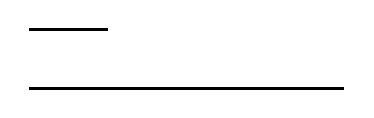
\begin{tikzpicture}[xkcd, line width=1.1pt]
  \draw (0,0.75) -- (1,0.75);
  \draw (0,0) -- (4,0);
\end{tikzpicture}}

\newcommand{\sizesquare}{%
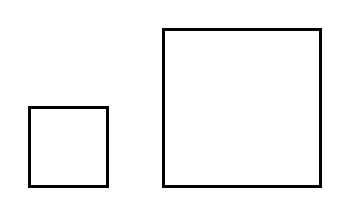
\begin{tikzpicture}[xkcd, line width=1.1pt]
  \draw (0,0) rectangle (1,1);
  \draw (1.7,0) rectangle (3.7,2);
\end{tikzpicture}}

\newcommand{\sizecircle}{%
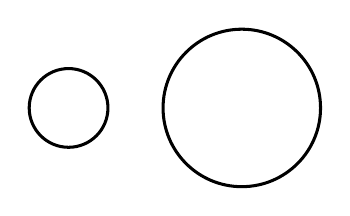
\begin{tikzpicture}[xkcd, line width=1.1pt]
  \draw (0,1) circle (0.5cm);
  \draw (2.2,1) circle (1cm);
\end{tikzpicture}}

\newcommand{\sizecube}{%
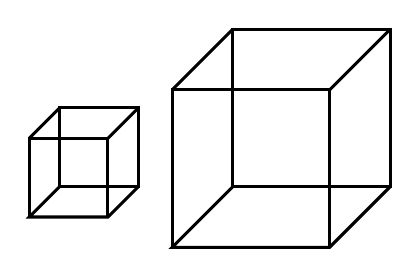
\begin{tikzpicture}[line width=1.1pt]
  \draw (0,0,0) -- (1,0,0) -- (1,1,0) -- (0,1,0) -- cycle;
  \draw (0,0,0) -- (0,0,1) -- (1,0,1) -- (1,0,0);
  \draw (1,0,1) -- (1,1,1) -- (0,1,1) -- (0,0,1);
  \draw (1,1,0) -- (1,1,1);
  \draw (0,1,0) -- (0,1,1);
  \begin{scope}[xshift=2.2cm, scale=2]
  \draw (0,0,0) -- (1,0,0) -- (1,1,0) -- (0,1,0) -- cycle;
  \draw (0,0,0) -- (0,0,1) -- (1,0,1) -- (1,0,0);
  \draw (1,0,1) -- (1,1,1) -- (0,1,1) -- (0,0,1);
  \draw (1,1,0) -- (1,1,1);
  \draw (0,1,0) -- (0,1,1);
  \end{scope}
\end{tikzpicture}}

% ---------------------------------------------------------------------------
% Part 2: the equal-bin chart. Five bins five hours wide, from 0 to 25.
% The y axis reaches 16 because one bin holds sixteen of the twenty people,
% which is the point of the picture.
% ---------------------------------------------------------------------------
\newcommand{\linbar}[3]{\draw[barstyle] (#1,0) rectangle (#2,#3);}

\newcommand{\linhist}[1]{%
\begin{tikzpicture}[x=0.47cm, y=0.36cm]
  \foreach \y in {4,8,12,16} \draw[gridline] (0,\y) -- (25.6,\y);
  \foreach \x in {5,10,15,20} \draw[binsep] (\x,0) -- (\x,17.5);
  #1
  \draw[axisline] (0,0) -- (26.4,0);
  \draw[axisline] (0,0) -- (0,17.5);
  \foreach \x in {0,5,10,15,20,25} {
    \draw[axisline] (\x,0) -- ++(0,-0.16cm);
    \node[tlab, below] at (\x,-0.55) {\x};}
  \foreach \y in {0,4,8,12,16} {
    \draw[axisline] (0,\y) -- ++(-0.16cm,0);
    \node[tlab, left] at (-0.4,\y) {\y};}
  \node[tlab] at (13,-3.7) {hours watched last week};
  \node[tlab, rotate=90] at (-3.4,8.75) {people};
\end{tikzpicture}}

% ---------------------------------------------------------------------------
% Part 3: the doubling-bin chart. Six bins, each drawn the same width, which
% is what a log axis is. Slot i runs from i to i+1.
% ---------------------------------------------------------------------------
\newcommand{\logbar}[2]{\draw[barstyle] (#1,0) rectangle (#1+1,#2);}

\newcommand{\loghist}[1]{%
\begin{tikzpicture}[x=1.78cm, y=0.45cm]
  \foreach \y in {2,4,6,8} \draw[gridline] (0,\y) -- (6.1,\y);
  \foreach \x in {1,2,3,4,5} \draw[binsep] (\x,0) -- (\x,9.3);
  #1
  \draw[axisline] (0,0) -- (6.3,0);
  \draw[axisline] (0,0) -- (0,9.3);
  \foreach \y in {0,2,4,6,8} {
    \draw[axisline] (0,\y) -- ++(-0.10cm,0);
    \node[tlab, left] at (-0.062,\y) {\y};}
  \foreach \x/\lab in {0/{0--1}, 1/{1--2}, 2/{2--4}, 3/{4--8},
                       4/{8--16}, 5/{16--32}} {
    \node[slab] at (\x+0.5,-0.95) {\lab};}
  \node[tlab] at (3,-2.5) {hours watched last week};
  \node[tlab, rotate=90] at (-0.60,4.65) {people};
\end{tikzpicture}}

% ---------------------------------------------------------------------------
% Part 3: the two rulers. Both are the same length on paper. The top one
% spreads 0 to 32 evenly; on the bottom one every step doubles.
% #1 is whatever gets marked on them.
% ---------------------------------------------------------------------------
\newcommand{\rulers}[1]{%
\begin{tikzpicture}[y=1cm]
  % Top: even spacing, 0 to 32 across 12cm.
  \draw[axisline] (0,3.6) -- (12.4,3.6);
  \foreach \n in {0,4,8,12,16,20,24,28,32} {
    \draw[axisline] (\n*0.375,3.6) -- ++(0,-0.24);
    \node[tlab, below] at (\n*0.375,3.36) {\n};}
  \node[tlab, anchor=west] at (0,4.65) {\bfseries Ruler A \normalfont ---
    every step adds 4};
  % Bottom: doubling, 1 to 32 across the same 12cm.
  \draw[axisline] (0,0) -- (12.4,0);
  \foreach \n/\p in {1/0, 2/1, 4/2, 8/3, 16/4, 32/5} {
    \draw[axisline] (\p*2.4,0) -- ++(0,-0.24);
    \node[tlab, below] at (\p*2.4,-0.24) {\n};}
  \node[tlab, anchor=west] at (0,0.5) {\bfseries Ruler B \normalfont ---
    every step doubles};
  #1
\end{tikzpicture}}

% ---------------------------------------------------------------------------
% Part 4: the doubling grid the five counted fractions are plotted on. Both
% rulers double, so five points that halve each time land on a straight line.
% Slot i on x is 1,2,4,8,16; slot j on y is 0.05,0.1,0.2,0.4,0.8.
% ---------------------------------------------------------------------------
\newcommand{\ccdfgrid}[1]{%
\begin{tikzpicture}[x=2.35cm, y=1.72cm]
  \foreach \j in {0,1,2,3,4} \draw[gridline] (0,\j) -- (4.3,\j);
  \foreach \i in {0,1,2,3,4} \draw[gridline] (\i,-0.3) -- (\i,4.3);
  #1
  % The axes sit clear of the lowest gridline, so the point that lands on
  % 0.05 is not drawn half underneath the axis.
  \draw[axisline] (-0.12,-0.3) -- (4.4,-0.3);
  \draw[axisline] (0,-0.42) -- (0,4.4);
  \foreach \i/\lab in {0/1, 1/2, 2/4, 3/8, 4/16} {
    \draw[axisline] (\i,-0.3) -- ++(0,-0.10cm);
    \node[tlab, below] at (\i,-0.385) {\lab};}
  \foreach \j/\lab in {0/{0.05}, 1/{0.1}, 2/{0.2}, 3/{0.4}, 4/{0.8}} {
    \draw[axisline] (0,\j) -- ++(-0.10cm,0);
    \node[tlab, left] at (-0.043,\j) {\lab};}
  \node[tlab] at (2,-1.15) {$k$ hours};
  \node[tlab, rotate=90] at (-0.66,1.85)
    {fraction watching more than $k$};
\end{tikzpicture}}

% ---------------------------------------------------------------------------
% The worked charts, used by solutions.tex only. They live here so that the
% blank grid and the filled one can never drift apart.
% ---------------------------------------------------------------------------
% Part 2: sixteen people in the first bin, three in the second, none in the
% next two, one at the far right.
\newcommand{\linsol}{%
  \linbar{0}{5}{16}\linbar{5}{10}{3}\linbar{20}{25}{1}}

% Part 3: 4, 8, 4, 2, 1, 1 -- every bar visible, and after the peak each one
% is half the one before.
\newcommand{\logsol}{%
  \logbar{0}{4}\logbar{1}{8}\logbar{2}{4}\logbar{3}{2}\logbar{4}{1}%
  \logbar{5}{1}}

% Part 3: where 5 lands on each ruler. On Ruler A that is 5/32 along; on
% Ruler B it is log2(5) = 2.32 steps of 2.4cm.
\newcommand{\fivemarks}{%
  \draw[marker] (1.875,3.98) -- (1.875,3.22);
  \node[tlab, pltblue!72!black, above] at (1.875,3.98) {\bfseries 5};
  \draw[marker] (5.573,0.38) -- (5.573,-0.38);
  \node[tlab, pltblue!72!black, above] at (5.573,0.38) {\bfseries 5};}

% Part 4: the five counted fractions. They halve as k doubles, so they land
% on one straight line.
\newcommand{\ccdfsol}{%
  \draw[marker, opacity=0.4] (0,4) -- (4,0);
  \foreach \i/\j in {0/4, 1/3, 2/2, 3/1, 4/0} {
    \node[ccdfdot] at (\i,\j) {};}}


% The twenty answers, smallest first. One list, so the sheet and its key can
% never disagree about the data.
\newcommand{\dsp}{\hspace{0.75em}}
\newcommand{\gotdata}{1\dsp 1\dsp 1\dsp 1\dsp 2\dsp 2\dsp 2\dsp 2\dsp 2\dsp
  2\dsp 2\dsp 2\dsp 3\dsp 3\dsp 4\dsp 4\dsp 6\dsp 7\dsp 10\dsp 24}


% An answer, set apart from the question it belongs to. Wrapped rather than
% switched: a bare \color inside a p-column cell costs the cell its first line.
\newcommand{\ans}[1]{\textbf{\textcolor{pltblue!75!black}{#1}}}

% The line that turns from question to answer.
\newcommand{\arrow}{\textcolor{pltblue!75!black}{$\Rightarrow$}\;}

% The same as \ans, for something already inside math: \ans wraps its argument
% in \textbf, which leaves math mode and takes the formula with it.
\newcommand{\mans}[1]{{\color{pltblue!75!black}#1}}

\begin{document}

\begin{center}
{\ppfont\LARGE Answers}
\end{center}

{\small The sheet with its answers, \ans{in blue}.}

\parthead{1}{Your eye is not a ruler}

{\bf Question 1(a)}: For each of the four pairs, how many times bigger is the
big one? Length for the lines, area for the square and the circle, volume for
the cube.

\arrow \ans{4, 4, 4, and 8.} The line is four times as long. The big square has
twice the side of the small one, so \ans{four times the area}. The big circle
has twice the radius, so again \ans{four times the area}. The big cube has
twice the edge, so \ans{eight times the volume}.

Only the first of those four is usually guessed right. Most people say about
2.5 for the two areas and about 3.5 for the cube --- roughly the true ratio
raised to the power 0.7 for an area and 0.6 for a volume, which is what a
century of experiments on the question keeps finding.

{\bf Question 1(b)}: On which pair were you and your neighbour furthest apart,
and why that pair?

\arrow \ans{The cube}, almost always. Your eye does not multiply. It reads
``how much wider'' and stops there, so the more directions a shape grows in,
the further the guess falls behind. Hold on to that: the rest of this sheet is
about twenty numbers that grow the same way, and about what a chart has to do
so that your eye is not fooled by them.

\parthead{2}{Twenty people and Game of Thrones}

Twenty people, asked how many hours they spent watching Game of Thrones last
week, smallest first:

\begin{center}\gotdata\end{center}

{\bf Question 2}: Count the twenty people into five bins, each five hours wide,
and darken a bar for each.

\arrow \ans{16, 3, 0, 0, 1}, drawn below left. Sixteen people watched five
hours or less; 6, 7 and 10 make the second bar; nobody is in the next two bins;
and the person who watched 24 hours is the last bar, alone.

\begin{center}
\begin{tabular}{@{}c@{\hspace{0.8cm}}c@{}}
\resizebox{0.46\textwidth}{!}{\linhist{\linsol}} &
\resizebox{0.46\textwidth}{!}{\loghist{\logsol}} \\[0.4em]
{\small\bfseries Question 2: equal bins} &
{\small\bfseries Question 4: doubling bins} \\
\end{tabular}
\end{center}

{\bf Question 3}: Put your thumb over the tallest bar. What can you still say
about the four people who watched more than five hours? And what does a
newspaper reader take away in two seconds?

\arrow \ans{Almost nothing.} Under your thumb are 80\% of the people, and what
is left is one short bar, two empty bins, and one bar of height 1 that is easy
to mistake for a printing error. You cannot see that three of the four watched
between 6 and 10 hours, and you certainly cannot see that one person watched
five times as much as anybody else.

The reader walks away with \ans{``nearly everybody watches under five
hours''} --- which is true, and which is the least interesting thing in the
data. The chart has spent its whole width on a fact that needed one sentence,
and has hidden the only surprising person in it.

\parthead{3}{Bins that double}

{\bf Question 4}: The same twenty numbers, counted into six bins, each twice as
wide as the one before.

\arrow \ans{4, 8, 4, 2, 1, 1}, drawn above right. The eight people on exactly
2 hours go in the 1--2 bin, by the sheet's boundary rule. Check the total:
still twenty people, not one of them moved. Only the bins changed.

{\bf Question 5}: In Part 2 sixteen of the twenty sat in one bar. What is the
biggest bar now, and what did the doubling bins do?

\arrow The biggest bar is \ans{8}, the 1--2 bin. The doubling bins
\ans{spread the twenty people over six bars that you can all see}, instead of
piling 80\% of them into one. Look at what the new chart shows that the old one
could not: after the peak, \ans{each bar is about half the one before it} ---
8, 4, 2, 1. That halving is the shape of the data, and Part 2's chart had it
too. It just had no room to draw it.

{\bf Question 6(a)}: Mark where 5 goes on each ruler.

\arrow Below. On Ruler A, 5 sits just past the 4 mark, about one sixth of the
way along. On Ruler B it sits between 4 and 8, a little to the \ans{left} of
the middle of that gap: the middle of a doubling step is not 6 but about 5.7,
the number you have to multiply 4 by twice to land on 8.

\begin{center}
\resizebox{0.88\textwidth}{!}{\rulers{\fivemarks}}
\end{center}

{\bf Question 6(b)}: Sixteen of your twenty watched between 1 and 4 hours. How
much of Ruler A do they get? How much of Ruler B? And why can Ruler B never be
given a 0?

\arrow On Ruler A, 1 to 4 is three units out of thirty-two ---
\ans{about a tenth} of the ruler, for 80\% of your people. On Ruler B it is two
steps out of five, \ans{40\%}. That is the whole trick, and it is the same
trick as Question 4: \ans{Ruler B is the doubling-bin chart's x-axis}, and a
chart drawn on it is called a \ans{log plot}.

Ruler B has no 0 because you reach the left end of it by halving --- 1, then
$\tfrac12$, then $\tfrac14$ --- and halving never arrives. \ans{Zero is
infinitely far to the left}, so a log axis cannot show it. Nothing that can be
zero, or negative, belongs on one.

\parthead{4}{Counting without bins}

{\bf Question 7}: One more person watched 12 hours --- which bar of Part 3
changes, and by what fraction of itself? Then one more who watched 2 hours
instead. Which bars would you trust?

\arrow The 12-hour person lands in the 8--16 bin, which goes from 1 to 2: that
bar \ans{doubles, +100\%}. The 2-hour person lands in the 1--2 bin, which goes
from 8 to 9: \ans{+12.5\%}.

So \ans{the tall bars on the left are steady and the short bars on the right
are not}. One extra person barely moves the left of the chart and can double
the right of it. That is a problem, because the right of the chart is the part
you actually wanted: the heavy watchers, the hubs, the rare and interesting
end. Widen the bins and the noise goes away, but so does the detail; narrow
them and every tail bar is one person again. \ans{There is no bin width that
fixes it}, which is why Part 4 stops choosing one.

\needroom{9\baselineskip}%
{\bf Question 8}: For each $k$, how many of the twenty watched more than $k$
hours?

\arrow Count from the right-hand end of the sorted list --- no bins, no
choices:

\begin{center}
{\setlength{\tabcolsep}{6pt}\renewcommand{\arraystretch}{1.3}
\begin{tabular}{|l|C{1.6cm}|C{1.6cm}|C{1.6cm}|C{1.6cm}|C{1.6cm}|}
\hline
$k$ hours & 1 & 2 & 4 & 8 & 16 \\
\hline
people watching more & 16 & \ans{8} & \ans{4} & \ans{2} & \ans{1} \\
\hline
as a fraction of 20 & 0.80 & \ans{0.40} & \ans{0.20} & \ans{0.10} & \ans{0.05} \\
\hline
\end{tabular}}
\end{center}

{\bf Question 9(a)}: Plot the five fractions on two doubling rulers. What do
the points do?

\arrow \ans{They fall on a straight line.}

\begin{center}
\resizebox{0.52\textwidth}{!}{\ccdfgrid{\ccdfsol}}
\end{center}

Every time the hours double, \ans{the number of people left halves}: 16, 8, 4,
2, 1. On two doubling rulers, ``double the one, halve the other'' is a straight
line at 45 degrees, and that is the only reason the five points line up.

The count you just made has a name --- it is the \ans{CCDF}, the fraction of
the data above $k$ --- and this picture is how every heavy-tailed measurement
in the course gets drawn. It never asked you for a bin.

{\bf Question 9(b)}: Someone counts the other way round: the fraction watching
$k$ hours \emph{or fewer}, which is 0.80 at $k = 4$, 0.90 at $k = 8$, 0.95 at
$k = 16$. What are those numbers doing, and which count shows you the 24-hour
person?

\arrow They \ans{creep towards 1 and flatten}, and they can never pass it. Both
counts hold exactly the same twenty numbers --- one is 1 minus the other ---
but this one squeezes every heavy watcher into the last thin sliver under the
ceiling, where the differences between 0.95 and 0.99 are invisible.

\ans{The ``more than'' count shows the 24-hour person}, as the last point on
the right, in its own place on the ruler. The ``or fewer'' count is the
\ans{CDF}; use it when you care about the typical case, and the CCDF when you
care about the tail.

{\bf Question 10}: The twenty people are now twenty nodes and each number is
how many friends that node has. How would you draw Question 9(a)'s picture for
a million nodes? And which of today's three pictures would you print?

\arrow For each $k$, \ans{count how many nodes have more than $k$ friends,
divide by a million, and plot that against $k$ with both axes doubling}.
Nothing in it grows with the network except the counting: no bin width to argue
about, no empty bars, and every node contributes to every point.

\ans{Print the third picture.} The first hides 80\% of the network in one bar;
the second shows the shape but wobbles by 100\% wherever the data is thin; the
third is the one you can read the tail off.

And the straight line is the thing you will spend the next lecture on. In a
network, ``how many friends'' is called \ans{degree}, the counts you drew are
the \ans{degree distribution}, and a degree distribution whose CCDF is a
straight line on doubling rulers is a \ans{power law}. Its slope is the one
number that says how rare the hubs are --- here, half as many people every time
you double, which is a slope of $\mans{-1}$.

One warning to carry with it, because Question 9(a) makes it look too easy:
five points on a line are five points on a line. A straight-looking log plot is
where the question starts, not where it is settled.

\end{document}
